% Options for packages loaded elsewhere
\PassOptionsToPackage{unicode}{hyperref}
\PassOptionsToPackage{hyphens}{url}
\PassOptionsToPackage{dvipsnames,svgnames*,x11names*}{xcolor}
%
\documentclass[
  english,
  man,floatsintext]{apa6}
\usepackage{lmodern}
\usepackage{amssymb,amsmath}
\usepackage{ifxetex,ifluatex}
\ifnum 0\ifxetex 1\fi\ifluatex 1\fi=0 % if pdftex
  \usepackage[T1]{fontenc}
  \usepackage[utf8]{inputenc}
  \usepackage{textcomp} % provide euro and other symbols
\else % if luatex or xetex
  \usepackage{unicode-math}
  \defaultfontfeatures{Scale=MatchLowercase}
  \defaultfontfeatures[\rmfamily]{Ligatures=TeX,Scale=1}
\fi
% Use upquote if available, for straight quotes in verbatim environments
\IfFileExists{upquote.sty}{\usepackage{upquote}}{}
\IfFileExists{microtype.sty}{% use microtype if available
  \usepackage[]{microtype}
  \UseMicrotypeSet[protrusion]{basicmath} % disable protrusion for tt fonts
}{}
\makeatletter
\@ifundefined{KOMAClassName}{% if non-KOMA class
  \IfFileExists{parskip.sty}{%
    \usepackage{parskip}
  }{% else
    \setlength{\parindent}{0pt}
    \setlength{\parskip}{6pt plus 2pt minus 1pt}}
}{% if KOMA class
  \KOMAoptions{parskip=half}}
\makeatother
\usepackage{xcolor}
\IfFileExists{xurl.sty}{\usepackage{xurl}}{} % add URL line breaks if available
\IfFileExists{bookmark.sty}{\usepackage{bookmark}}{\usepackage{hyperref}}
\hypersetup{
  pdftitle={Epidemiologische situatie COVID-19 in Nederland - 27 december 2021},
  pdfauthor={Marino van Zelst1},
  pdflang={en-EN},
  colorlinks=true,
  linkcolor=Maroon,
  filecolor=Maroon,
  citecolor=Blue,
  urlcolor=blue,
  pdfcreator={LaTeX via pandoc}}
\urlstyle{same} % disable monospaced font for URLs
\usepackage{graphicx,grffile}
\makeatletter
\def\maxwidth{\ifdim\Gin@nat@width>\linewidth\linewidth\else\Gin@nat@width\fi}
\def\maxheight{\ifdim\Gin@nat@height>\textheight\textheight\else\Gin@nat@height\fi}
\makeatother
% Scale images if necessary, so that they will not overflow the page
% margins by default, and it is still possible to overwrite the defaults
% using explicit options in \includegraphics[width, height, ...]{}
\setkeys{Gin}{width=\maxwidth,height=\maxheight,keepaspectratio}
% Set default figure placement to htbp
\makeatletter
\def\fps@figure{htbp}
\makeatother
\setlength{\emergencystretch}{3em} % prevent overfull lines
\providecommand{\tightlist}{%
  \setlength{\itemsep}{0pt}\setlength{\parskip}{0pt}}
\setcounter{secnumdepth}{-\maxdimen} % remove section numbering
% Make \paragraph and \subparagraph free-standing
\ifx\paragraph\undefined\else
  \let\oldparagraph\paragraph
  \renewcommand{\paragraph}[1]{\oldparagraph{#1}\mbox{}}
\fi
\ifx\subparagraph\undefined\else
  \let\oldsubparagraph\subparagraph
  \renewcommand{\subparagraph}[1]{\oldsubparagraph{#1}\mbox{}}
\fi
% Manuscript styling
\usepackage{upgreek}
\captionsetup{font=singlespacing,justification=justified}

% Table formatting
\usepackage{longtable}
\usepackage{lscape}
% \usepackage[counterclockwise]{rotating}   % Landscape page setup for large tables
\usepackage{multirow}		% Table styling
\usepackage{tabularx}		% Control Column width
\usepackage[flushleft]{threeparttable}	% Allows for three part tables with a specified notes section
\usepackage{threeparttablex}            % Lets threeparttable work with longtable

% Create new environments so endfloat can handle them
% \newenvironment{ltable}
%   {\begin{landscape}\begin{center}\begin{threeparttable}}
%   {\end{threeparttable}\end{center}\end{landscape}}
\newenvironment{lltable}{\begin{landscape}\begin{center}\begin{ThreePartTable}}{\end{ThreePartTable}\end{center}\end{landscape}}

% Enables adjusting longtable caption width to table width
% Solution found at http://golatex.de/longtable-mit-caption-so-breit-wie-die-tabelle-t15767.html
\makeatletter
\newcommand\LastLTentrywidth{1em}
\newlength\longtablewidth
\setlength{\longtablewidth}{1in}
\newcommand{\getlongtablewidth}{\begingroup \ifcsname LT@\roman{LT@tables}\endcsname \global\longtablewidth=0pt \renewcommand{\LT@entry}[2]{\global\advance\longtablewidth by ##2\relax\gdef\LastLTentrywidth{##2}}\@nameuse{LT@\roman{LT@tables}} \fi \endgroup}

% \setlength{\parindent}{0.5in}
% \setlength{\parskip}{0pt plus 0pt minus 0pt}

% \usepackage{etoolbox}
\makeatletter
\patchcmd{\HyOrg@maketitle}
  {\section{\normalfont\normalsize\abstractname}}
  {\section*{\normalfont\normalsize\abstractname}}
  {}{\typeout{Failed to patch abstract.}}
\patchcmd{\HyOrg@maketitle}
  {\section{\protect\normalfont{\@title}}}
  {\section*{\protect\normalfont{\@title}}}
  {}{\typeout{Failed to patch title.}}
\makeatother
\shorttitle{Dagelijkse rapportage}
\DeclareDelayedFloatFlavor{ThreePartTable}{table}
\DeclareDelayedFloatFlavor{lltable}{table}
\DeclareDelayedFloatFlavor*{longtable}{table}
\makeatletter
\renewcommand{\efloat@iwrite}[1]{\immediate\expandafter\protected@write\csname efloat@post#1\endcsname{}}
\makeatother
\usepackage{csquotes}
\ifxetex
  % Load polyglossia as late as possible: uses bidi with RTL langages (e.g. Hebrew, Arabic)
  \usepackage{polyglossia}
  \setmainlanguage[]{english}
\else
  \usepackage[shorthands=off,main=english]{babel}
\fi

\title{Epidemiologische situatie COVID-19 in Nederland - 27 december 2021}
\author{Marino van Zelst\textsuperscript{1}}
\date{}


\affiliation{\vspace{0.5cm}\textsuperscript{1} Vragen over deze rapportage kunnen verstuurd worden aan Marino van Zelst, twitter.com/mzelst. E-mail: \href{mailto:j.m.vanzelst@uvt.nl}{\nolinkurl{j.m.vanzelst@uvt.nl}}}

\begin{document}
\maketitle

{
\hypersetup{linkcolor=}
\setcounter{tocdepth}{3}
\tableofcontents
}
\newpage

\hypertarget{samenvatting}{%
\section{Samenvatting}\label{samenvatting}}

\textbf{Samenvatting (op basis van GGD cijfers)}\\
Tot en met 2021-12-27 zijn er in Nederland in totaal 3076442 COVID-19 patiënten gemeld aan het RIVM. Tot nu toe zijn 37477 van de gemelde patiënten opgenomen in het ziekenhuis en 20728 mensen overleden.

\textbf{Gegevens t. o. v. gisteren}\\
Positief getest: 11495
Totaal: 3076442 (+ 11432 ivm -63 corr.)

Opgenomen: 41
Totaal: 37477 (+
39 ivm -2 corr.)

Overleden: 12
Totaal: 20728 (+
12 ivm 0 corr.)

\textbf{Update met betrekking tot ziekenhuis-gegevens (data NICE)}

Patiënten verpleegafdeling\\
Bevestigd: 20 Verdacht: 4

Patiënten IC\\
Bevestigd: 9 Verdacht: 0

\textbf{Data}\\
Een databestand met de cumulatieve aantallen per gemeente per dag van gemelde COVID-19 patiënten, in het ziekenhuis opgenomen COVID-19 patiënten en overleden COVID-19 patiënten is \href{https://data.rivm.nl/geonetwork/srv/dut/catalog.search\#/metadata/1c0fcd57-1102-4620-9cfa-441e93ea5604}{hier} te vinden. Een databestand met karakteristieken van elke positief geteste COVID-19 patiënt in Nederland is \href{https://data.rivm.nl/geonetwork/srv/dut/catalog.search\#/metadata/2c4357c8-76e4-4662-9574-1deb8a73f724?tab=relations}{hier} te vinden. Alle gegevens die voor dit rapport gebruikt worden zijn te vinden in de \href{https://github.com/mzelst/covid-19}{Github repository}.

\newpage

\hypertarget{covid-19-meldingen-in-de-afgelopen-vier-weken}{%
\section{COVID-19 meldingen in de afgelopen vier weken}\label{covid-19-meldingen-in-de-afgelopen-vier-weken}}

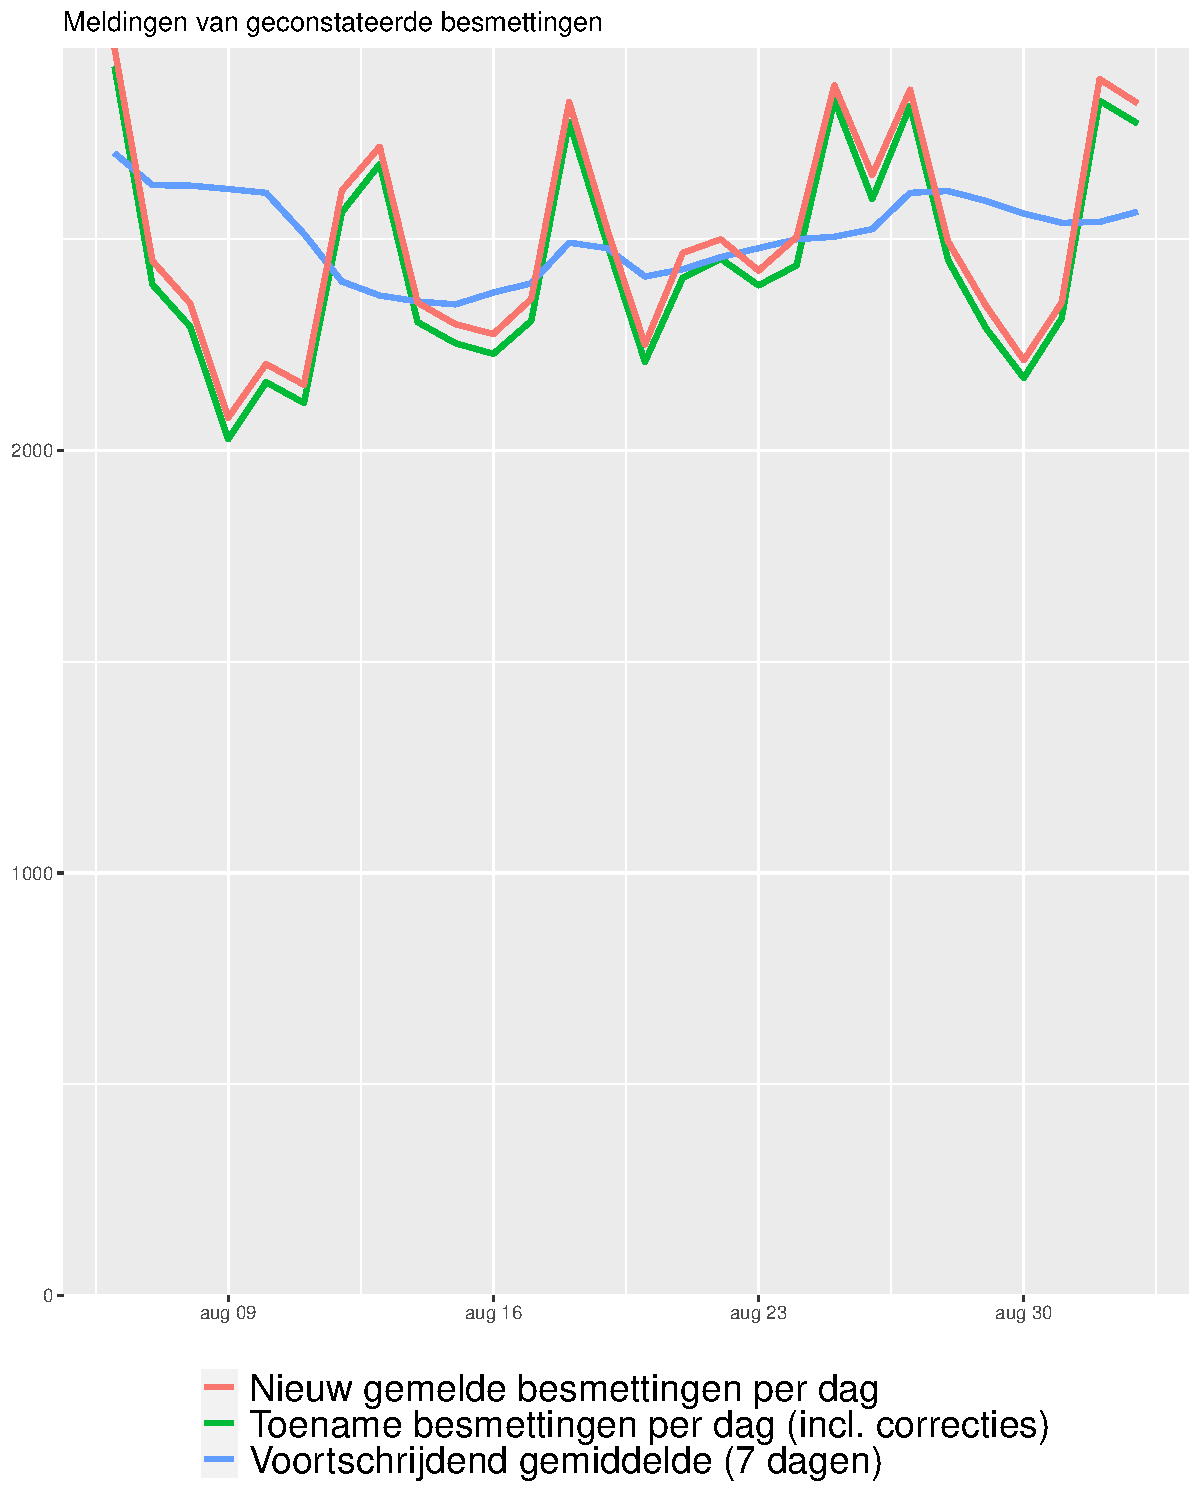
\includegraphics{daily_report_files/figure-latex/Gemelde besmettingen-1.pdf}

\newpage

\hypertarget{kaart-met-covid-19-meldingen-per-gemeente-sinds-gisteren}{%
\section{Kaart met COVID-19 meldingen per gemeente sinds gisteren}\label{kaart-met-covid-19-meldingen-per-gemeente-sinds-gisteren}}

\begin{figure}
\centering
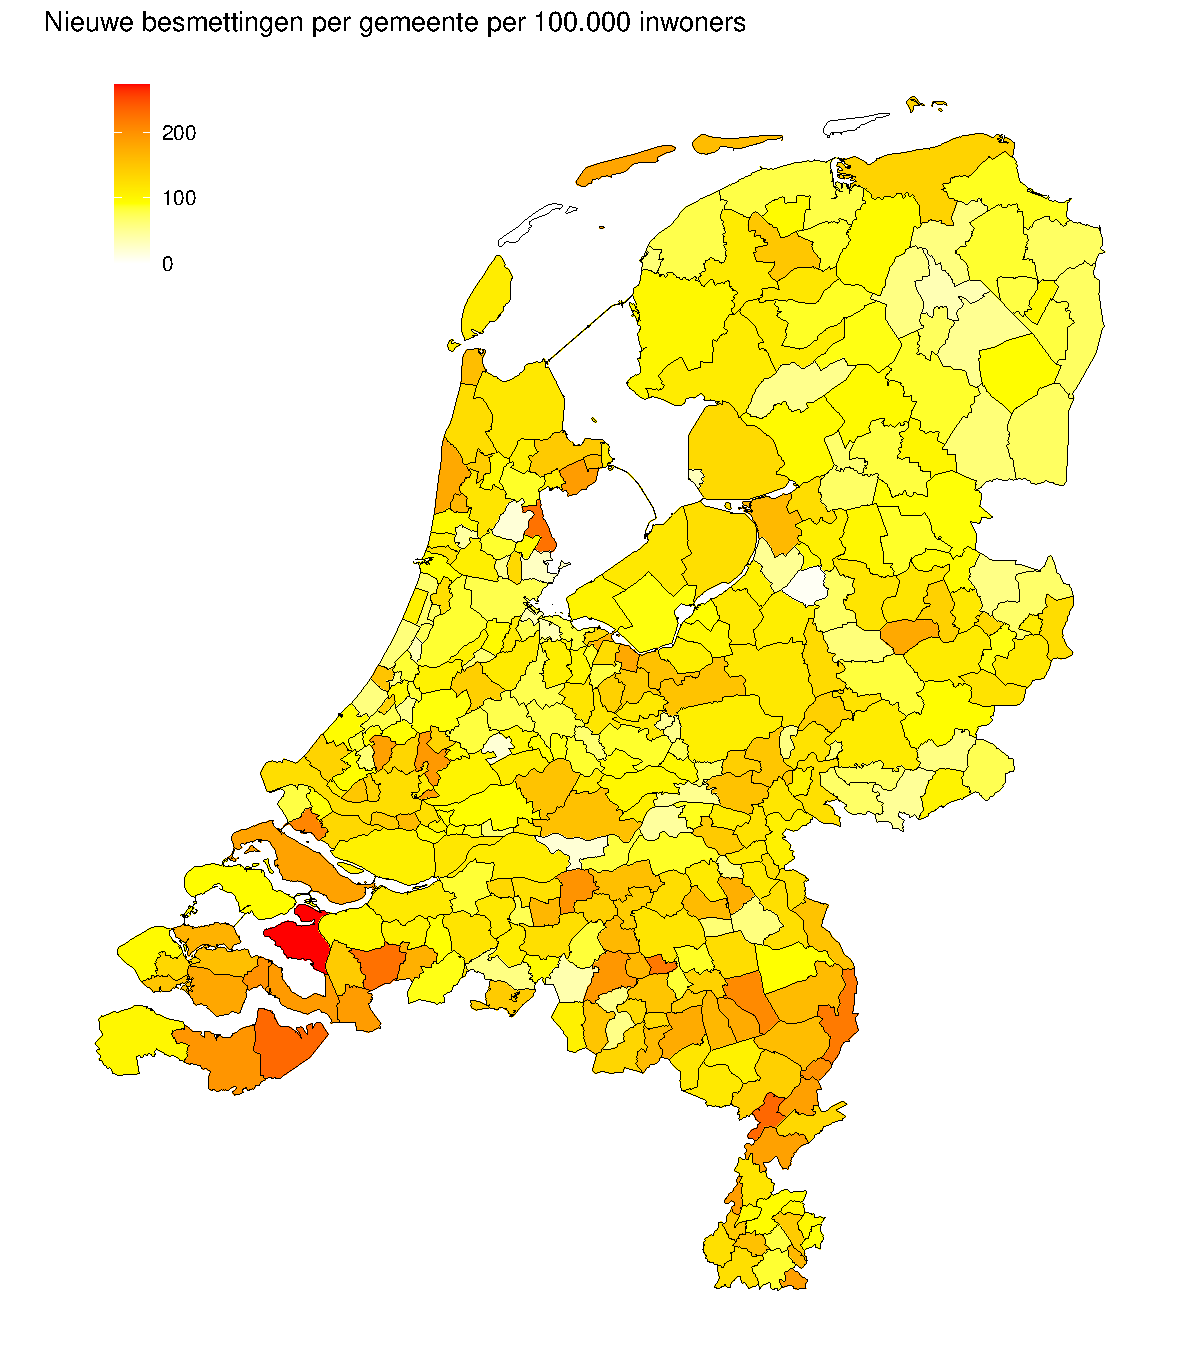
\includegraphics{daily_report_files/figure-latex/Gemeentes - sinds gisteren-1.pdf}
\caption{(\#Gemeentes - sinds gisteren) Aantal, sinds gisteren, bij de GGD'en gemelde COVID-19 patiënten per 100.000 inwoners per gemeente}
\end{figure}

\newpage

\hypertarget{kaart-met-covid-19-meldingen-per-gemeente-in-de-afgelopen-week}{%
\section{Kaart met COVID-19 meldingen per gemeente in de afgelopen week}\label{kaart-met-covid-19-meldingen-per-gemeente-in-de-afgelopen-week}}

\begin{figure}
\centering
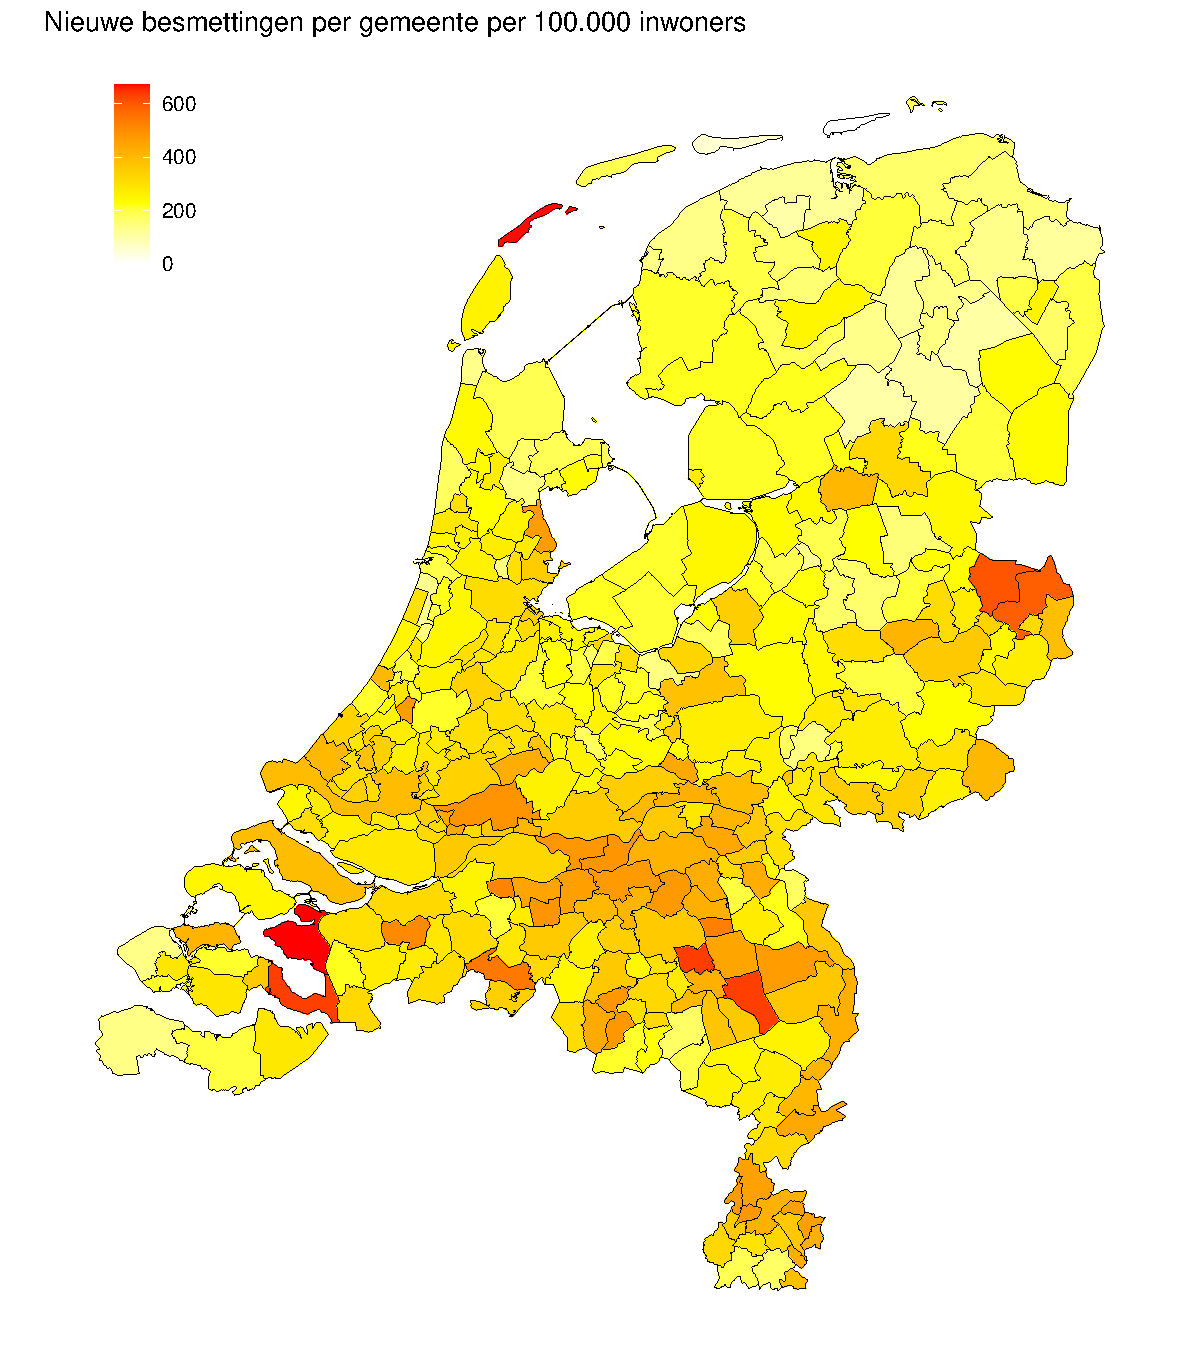
\includegraphics{daily_report_files/figure-latex/Gemeentes - Sinds vorige week-1.pdf}
\caption{(\#Gemeentes - Sinds vorige week) Aantal in de afgelopen week bij de GGD'en gemelde COVID-19 patiënten per 100.000 inwoners per gemeente.}
\end{figure}

\newpage

\hypertarget{aantal-covid-19-meldingen-per-provincie-in-de-afgelopen-twee-weken}{%
\section{Aantal COVID-19 meldingen per provincie in de afgelopen twee weken}\label{aantal-covid-19-meldingen-per-provincie-in-de-afgelopen-twee-weken}}

\begin{table}
\centering
\begin{threeparttable}
\begin{tabular}{lrrrrrr}
\toprule
\multicolumn{1}{c}{ } & \multicolumn{2}{c}{Besmettingen} & \multicolumn{2}{c}{Ziekenhuisopnames} & \multicolumn{2}{c}{Overleden} \\
\cmidrule(l{3pt}r{3pt}){2-3} \cmidrule(l{3pt}r{3pt}){4-5} \cmidrule(l{3pt}r{3pt}){6-7}
Provincie & Totaal & /100000 & Totaal & /100000 & Totaal & /100000\\
\midrule
Drenthe & 4450 & 894.6 & 14 & 2.8 & 8 & 1.6\\
Flevoland & 4918 & 1134.6 & 17 & 3.9 & 8 & 1.8\\
Fryslân & 7485 & 1144.6 & 28 & 4.3 & 31 & 4.7\\
Gelderland & 19545 & 927.0 & 88 & 4.2 & 102 & 4.8\\
Groningen & 4919 & 833.7 & 22 & 3.7 & 11 & 1.9\\
Limburg & 11985 & 1071.3 & 73 & 6.5 & 48 & 4.3\\
Noord-Brabant & 26595 & 1027.0 & 99 & 3.8 & 76 & 2.9\\
Noord-Holland & 32224 & 1110.4 & 137 & 4.7 & 99 & 3.4\\
Overijssel & 10776 & 920.4 & 39 & 3.3 & 37 & 3.2\\
Utrecht & 15068 & 1101.8 & 37 & 2.7 & 45 & 3.3\\
Zeeland & 4555 & 1177.7 & 67 & 17.3 & 13 & 3.4\\
Zuid-Holland & 39713 & 1059.9 & 184 & 4.9 & 110 & 2.9\\
\bottomrule
\end{tabular}
\begin{tablenotes}
\item \textit{Note: } 
\item Aantal bij de GGD’en gemelde COVID-19 patiënten, in het ziekenhuis opgenomen COVID-19 patiënten en overleden COVID-19 patiënten per provincie van 13 december t/m 27 december 10:00 uur, totaal en per 100.000 inwoners
\end{tablenotes}
\end{threeparttable}
\end{table}

\newpage

\hypertarget{aantal-covid-19-meldingen-per-ggd-in-de-afgelopen-twee-weken}{%
\section{Aantal COVID-19 meldingen per GGD in de afgelopen twee weken}\label{aantal-covid-19-meldingen-per-ggd-in-de-afgelopen-twee-weken}}

\begin{table}
\centering\begingroup\fontsize{10}{12}\selectfont

\begin{threeparttable}
\begin{tabular}{lrrrrrr}
\toprule
\multicolumn{1}{c}{ } & \multicolumn{2}{c}{Besmettingen} & \multicolumn{2}{c}{Ziekenhuisopnames} & \multicolumn{2}{c}{Overleden} \\
\cmidrule(l{3pt}r{3pt}){2-3} \cmidrule(l{3pt}r{3pt}){4-5} \cmidrule(l{3pt}r{3pt}){6-7}
GGD & Totaal & /100000 & Totaal & /100000 & Totaal & /100000\\
\midrule
Dienst Gezondheid \& Jeugd ZHZ & 5065 & 1093.1 & 12 & 2.6 & 19 & 4.1\\
GGD Amsterdam & 11858 & 1095.4 & 45 & 4.2 & 32 & 3.0\\
GGD Brabant-Zuidoost & 8047 & 1018.0 & 38 & 4.8 & 36 & 4.6\\
GGD Drenthe & 4451 & 894.3 & 14 & 2.8 & 7 & 1.4\\
GGD Flevoland & 4919 & 1133.3 & 17 & 3.9 & 8 & 1.8\\
GGD Fryslân & 7519 & 1149.2 & 29 & 4.4 & 31 & 4.7\\
GGD Gelderland-Zuid & 5153 & 906.4 & 16 & 2.8 & 21 & 3.7\\
GGD Gooi en Vechtstreek & 3130 & 1200.7 & 18 & 6.9 & 2 & 0.8\\
GGD Groningen & 4769 & 807.3 & 22 & 3.7 & 10 & 1.7\\
GGD Haaglanden & 11510 & 1016.9 & 86 & 7.6 & 33 & 2.9\\
GGD Hart voor Brabant & 11101 & 1021.4 & 31 & 2.9 & 29 & 2.7\\
GGD Hollands-Midden & 8051 & 981.6 & 29 & 3.5 & 16 & 2.0\\
GGD Hollands-Noorden & 7359 & 1099.1 & 26 & 3.9 & 26 & 3.9\\
GGD IJsselland & 5101 & 948.7 & 19 & 3.5 & 16 & 3.0\\
GGD Kennemerland & 6197 & 1119.5 & 30 & 5.4 & 29 & 5.2\\
GGD Limburg-Noord & 5243 & 1000.1 & 21 & 4.0 & 21 & 4.0\\
GGD Noord- en Oost-Gelderland & 8029 & 961.7 & 43 & 5.2 & 45 & 5.4\\
GGD Regio Utrecht & 15088 & 1102.2 & 37 & 2.7 & 46 & 3.4\\
GGD Rotterdam-Rijnmond & 15113 & 1131.9 & 58 & 4.3 & 43 & 3.2\\
GGD Twente & 5693 & 898.2 & 20 & 3.2 & 21 & 3.3\\
GGD West-Brabant & 7489 & 1048.2 & 29 & 4.1 & 13 & 1.8\\
GGD Zaanstreek/Waterland & 3680 & 1080.8 & 16 & 4.7 & 11 & 3.2\\
GGD Zeeland & 4549 & 1175.8 & 67 & 17.3 & 13 & 3.4\\
GGD Zuid-Limburg & 6760 & 1135.9 & 52 & 8.7 & 26 & 4.4\\
Veiligheids- en Gezondheidsregio Gelderland-Midden & 6359 & 900.2 & 30 & 4.2 & 34 & 4.8\\
\bottomrule
\end{tabular}
\begin{tablenotes}
\item \textit{Note: } 
\item Aantal bij de GGD’en gemelde COVID-19 patiënten, in het ziekenhuis opgenomen COVID-19 patiënten en overleden COVID-19 patiënten per GGD van 13 december t/m 27 december 10:00 uur, totaal en per 100.000 inwoners
\end{tablenotes}
\end{threeparttable}
\endgroup{}
\end{table}

\newpage

\hypertarget{ziekenhuisopnames-nice-in-de-afgelopen-twee-weken}{%
\section{Ziekenhuisopnames (NICE) in de afgelopen twee weken}\label{ziekenhuisopnames-nice-in-de-afgelopen-twee-weken}}

\begin{table}
\centering\begingroup\fontsize{10}{12}\selectfont

\begin{threeparttable}
\begin{tabular}{lrrrrrr}
\toprule
\multicolumn{1}{c}{ } & \multicolumn{2}{c}{Aanwezig} & \multicolumn{2}{c}{Opnames} & \multicolumn{2}{c}{Overleden} \\
\cmidrule(l{3pt}r{3pt}){2-3} \cmidrule(l{3pt}r{3pt}){4-5} \cmidrule(l{3pt}r{3pt}){6-7}
Leeftijd & Kliniek & IC & Kliniek & IC & Kliniek & IC\\
\midrule
<20 & 43 & 4 & 77 & 2 & -1 & 1\\
20 - 24 & 4 & 4 & 15 & 3 & 0 & 0\\
25 - 29 & 19 & 4 & 41 & 2 & 1 & 0\\
30 - 34 & 23 & 8 & 61 & 14 & 1 & 2\\
35 - 39 & 29 & 10 & 64 & 17 & 0 & 1\\
40 - 44 & 22 & 17 & 52 & 19 & 1 & 1\\
45 - 49 & 35 & 34 & 81 & 25 & 0 & 5\\
50 - 54 & 92 & 55 & 135 & 36 & 2 & 5\\
55 - 59 & 100 & 74 & 162 & 55 & 6 & 14\\
60 - 64 & 111 & 99 & 207 & 79 & 20 & 16\\
65 - 69 & 155 & 94 & 262 & 65 & 29 & 30\\
70 - 74 & 199 & 84 & 334 & 64 & 65 & 35\\
75 - 79 & 220 & 50 & 304 & 46 & 88 & 24\\
80 - 84 & 202 & 3 & 304 & 9 & 101 & 6\\
85 - 89 & 120 & 0 & 182 & 3 & 85 & 1\\
>90 & 44 & 0 & 79 & 0 & 35 & 1\\
\bottomrule
\end{tabular}
\begin{tablenotes}
\item \textit{Note: } 
\item Aantal bij NICE gemelde COVID-19 patiënten: in het ziekenhuis aanwezige COVID-19 patiënten, opnames, en overleden COVID-19 patiënten in het ziekenhuis van 13 december t/m 27 december 15:15 uur
\end{tablenotes}
\end{threeparttable}
\endgroup{}
\end{table}

\newpage

\hypertarget{leeftijdsverdeling-en-man-vrouwverdeling-van-covid-19-patiuxebnten-in-de-afgelopen-twee-weken}{%
\section{Leeftijdsverdeling en man-vrouwverdeling van COVID-19 patiënten in de afgelopen twee weken}\label{leeftijdsverdeling-en-man-vrouwverdeling-van-covid-19-patiuxebnten-in-de-afgelopen-twee-weken}}

\begin{table}
\centering\begingroup\fontsize{11}{13}\selectfont

\begin{threeparttable}
\begin{tabular}{lrrrrrr}
\toprule
\multicolumn{1}{c}{ } & \multicolumn{2}{c}{Besmettingen} & \multicolumn{2}{c}{Ziekenhuisopnames} & \multicolumn{2}{c}{Overleden} \\
\cmidrule(l{3pt}r{3pt}){2-3} \cmidrule(l{3pt}r{3pt}){4-5} \cmidrule(l{3pt}r{3pt}){6-7}
Leeftijdsgroep & Totaal & \% & Totaal & \% & Totaal & \%\\
\midrule
<50 & 10 & 0.0 & 7 & 0.9 & 10 & 1.7\\
0-9 & 22763 & 12.5 & 25 & 3.1 & NA & NA\\
10-19 & 25337 & 13.9 & 9 & 1.1 & NA & NA\\
20-29 & 27704 & 15.2 & 16 & 2.0 & NA & NA\\
30-39 & 30697 & 16.8 & 32 & 4.0 & NA & NA\\
40-49 & 26733 & 14.7 & 40 & 5.0 & NA & NA\\
50-59 & 21363 & 11.7 & 100 & 12.4 & 8 & 1.4\\
60-69 & 15209 & 8.3 & 174 & 21.6 & 41 & 7.0\\
70-79 & 8241 & 4.5 & 224 & 27.8 & 134 & 22.8\\
80-89 & 3246 & 1.8 & 144 & 17.9 & 238 & 40.5\\
90+ & 930 & 0.5 & 34 & 4.2 & 157 & 26.7\\
\bottomrule
\end{tabular}
\begin{tablenotes}
\item[1] Leeftijdsverdeling van bij de GGD’en gemelde COVID-19 patiënten, in het ziekenhuis opgenomen COVID-19 patiënten en overleden COVID-19 patiënten van 13 december t/m 27 december 10:00 uur.
\item[2] Overlijdensgevallen van patiënten jonger dan 50 jaar oud worden door het RIVM in de casusdata gegroepeerd in de categorie <50. Deze overlijdensgevallen zijn hier dus niet zichtbaar in deze leeftijdsgroepen maar alleen via de groep '<50'.
\end{tablenotes}
\end{threeparttable}
\endgroup{}
\end{table}

\newpage

\begin{table}
\centering\begingroup\fontsize{11}{13}\selectfont

\begin{threeparttable}
\begin{tabular}{lrrrrrr}
\toprule
\multicolumn{1}{c}{ } & \multicolumn{2}{c}{Besmettingen} & \multicolumn{2}{c}{Ziekenhuisopnames} & \multicolumn{2}{c}{Overleden} \\
\cmidrule(l{3pt}r{3pt}){2-3} \cmidrule(l{3pt}r{3pt}){4-5} \cmidrule(l{3pt}r{3pt}){6-7}
Geslacht & Totaal & \% & Totaal & \% & Totaal & \%\\
\midrule
Vrouw & 92898 & 51 & 348 & 43.2 & 281 & 47.8\\
Man & 89335 & 49 & 457 & 56.8 & 307 & 52.2\\
Onbekend & 0 & 0 & 0 & 0.0 & NA & NA\\
\bottomrule
\end{tabular}
\begin{tablenotes}
\item \textit{Note: } 
\item Man-vrouwverdeling van bij de GGD’en gemelde COVID-19 patiënten, in het ziekenhuis opgenomen COVID-19 patiënten en overleden COVID-19 patiënten van 13 december t/m 27 december 10:00 uur.
\end{tablenotes}
\end{threeparttable}
\endgroup{}
\end{table}
\newpage


\end{document}
